% Chapter 13: The birth and death chain of the zeros. Sources: misc/reviews/nick-volume3/vol3/ch6_birth_death.tex lines 1-57, 189-229, 284-312, 314-349, 351-464, 466-674, 676-864, 866-906, 908-939, 973-1048, 1050-1102; referee report U06 (M1 to M13), verification W3 (V8, V9). 17 Nov 2026.
\label{b:ch:chain}

\noindent
Volume II reads the Taylor coefficients of $\xi$ at the centre as a Stieltjes continued fraction, and the positivity of its coefficients as a Hankel test (Section~\ref{sec:ch21:hankel}). This chapter reads the same coefficients as the birth and death rates of a chain in the sense of Karlin and McGregor \cite{KarlinMcGregor57}, a reading already made in Section~\ref{ev:sec:string}, and asks what the chain looks like at depth. The material is from an unrefereed note of Polson (November 2026). The criterion itself is in the book: RH holds if and only if every rate is positive (Theorem~\ref{mw:thm:stieltjes}, Theorem~\ref{thm:ch12:inertia}, and the paragraph of Grommer and Chebotarev after it). For the classical diffusions the construction returns the continued fractions of Lambert and Gauss in closed form. For $\xi$ no closed form is known. We compute the chain from the moments of P\'olya's kernel and from the zeros, split the rates into a factor that depends on the Gamma factor alone and an arithmetic fluctuation, state the semiclassical law of the first factor as a heuristic, and run the same chain for $L(s,\chi_{12})$ and for the Davenport and Heilbronn function. The last section says what this does and does not give as a path to RH. Table~\ref{b:tab:summary} lists the results with their status.

\paragraph{Normalisation.} We use the notation of Volume II: $G(u)=\xi(\frac12+\sqrt u)/\xi(\frac12)$, the Thorin atoms are $\gamma_k^{-2}$, and the rates are the coefficients $c_j$ of
\begin{equation}\label{b:eq:Sfrac}
\frac{G'(u)}{G(u)}=\cfrac{m_0}{1+\cfrac{c_1u}{1+\cfrac{c_2u}{1+\cdots}}},\qquad m_0=\sum_{\gamma>0}\gamma^{-2}=0.0231049931154 .
\end{equation}
The coefficients with odd index are the birth rates and those with even index the death rates, and level $n$ means the first $2n-1$ coefficients, which is the Jacobi matrix of order $n$ of $\nu=\sum_k\gamma_k^{-2}\delta_{\gamma_k^{-2}}$. Positivity of $c_1,\dots,c_{2N-1}$ is positive definiteness of the Hankel matrices $\mathcal H_N(0)$ and $\mathcal H_N'(0)$ of Section~\ref{sec:ch21:hankel}. The note of Polson scales $G$ so that its rates are twice ours and its atoms are $2\gamma_k^{-2}$.

\begin{table}[ht]
\centering\small
\begin{tabular}{@{}p{3.4in}p{1.9in}@{}}
\toprule
Result & Status\\
\midrule
RH if and only if all $c_j>0$ (cited, Volume II) & proved\\
Closed form chains for Bessel hitting times, Proposition~\ref{b:prop:bessel} & proved (Lambert, Gauss)\\
Zeros recovered from the chain, Computation~\ref{b:comp:zeros} & computed\\
Level $n$ detects a pair above zero about $n/2$, Section~\ref{b:sec:toy} & computed\\
$c_j=c_j^\Gamma(1+\varepsilon_j)$, $|\varepsilon_j|\le0.15$, Computation~\ref{b:comp:deep} & computed (zeros real on the range)\\
Law $c_j^\Gamma=1/(4H_j^2)$, Conjecture~\ref{b:conj:bs} & heuristic; Abel inversion proved\\
$c_j^\Gamma\gamma_j^2\to\pi^2/4$, Corollary~\ref{b:cor:limit} & follows from the law\\
Candidate prime formula for $\varepsilon_j$, Section~\ref{b:sec:prime} & heuristic, rejected by computation\\
Spectral lines and dispersion clock, Conjecture~\ref{b:conj:ap} & computed; conjecture\\
Chain of $L(s,\chi_{12})$, Section~\ref{b:sec:eta} & computed\\
Davenport and Heilbronn control, Section~\ref{b:sec:dh} & computed\\
\bottomrule
\end{tabular}
\caption{Results of the chapter.}\label{b:tab:summary}
\end{table}

\section{Solvable models: Lambert and Gauss}

For the classical hitting times the chain is known in closed form, and it is the oldest continued fraction in analysis.

\begin{proposition}\label{b:prop:bessel}
Let $T$ be the time for a Bessel process of dimension $\delta$ started at $0$ to reach $1$, put $G(u)=1/\E e^{-uT/2}$, and let $\nu_B=\frac\delta2-1$. Then $G(u)=\Gamma(\nu_B+1)(2/\sqrt u)^{\nu_B}I_{\nu_B}(\sqrt u)$ and
\[
c_j=\frac{1}{4(\nu_B+j)(\nu_B+j+1)},\qquad j\ge1 .
\]
In particular $c_j=1/((2j-1)(2j+1))$ for reflected Brownian motion, where $G=\cosh\sqrt u$, and $c_j=1/((2j+1)(2j+3))$ for the Bessel(3) process, where $G=\sinh\sqrt u/\sqrt u$.
\end{proposition}
\begin{proof}
Put $w=\sqrt u$. Since $\frac{d}{dw}\log(w^{-\nu}I_\nu(w))=I_{\nu+1}(w)/I_\nu(w)$ and $\frac{d}{du}=\frac1{2w}\frac{d}{dw}$, we have $G'/G=I_{\nu+1}(w)/(2wI_\nu(w))$. Gauss' continued fraction
\[
\frac{I_{\nu+1}(w)}{I_\nu(w)}
=\cfrac{w}{2(\nu+1)+\cfrac{w^2}{2(\nu+2)+\cfrac{w^2}{2(\nu+3)+\cdots}}}
\]
with $w^2=u$, brought to the form \eqref{b:eq:Sfrac}, gives the stated coefficients. For $\nu=-\frac12$ it is Lambert's continued fraction $\tanh w/w=1/(1+w^2/(3+w^2/(5+\cdots)))$.
\end{proof}

So Lambert's continued fraction for the tangent is the chain of reflected Brownian motion. In these models the rates decay like $1/(4j^2)$, birth and death rates are nearly equal, and the $j$th coefficient tracks the $j$th zero: with $x_j=j_{\nu_B,j}^{-2}$ the $j$th atom of $\nu$,
\begin{equation}\label{b:eq:pi4}
\frac{c_j}{x_j}\ \longrightarrow\ \frac{\pi^2}{4}\qquad(j\to\infty),
\end{equation}
for every $\nu_B$, because $j_{\nu_B,j}\sim\pi j$. The two special cases are reproduced to twelve digits or better by the numerical chain (computed). By the criterion of Volume II, RH is the statement that $\xi'/\xi(\frac12+w)/w$ has a continued fraction of Lambert's type in $w^2$ with positive coefficients.

\section{Zeros from moments}

The level $n$ chain is the $n$ by $n$ Jacobi matrix with diagonal $a_0,\dots,a_{n-1}$ and off diagonal $\sqrt{b_1},\dots,\sqrt{b_{n-1}}$ of $\nu$ (the parameters $\alpha_n=c_{2n-2}+c_{2n-1}$, $\beta_n^2=c_{2n-1}c_{2n}$ of Section~\ref{sec:ch21:hankel}). Its eigenvalues are the nodes of the Gauss quadrature of $\nu$, and each eigenvalue $x$ gives an estimate $1/\sqrt x$ of a zero.

\begin{remark}[Computation: zeros from the chain]\label{b:comp:zeros}
The level $234$ chain reproduces the first $126$ zeros to six decimals, up to height $279.23$, and the first $121$ to twelve decimals (computed). At small levels:

\smallskip
\begin{center}\small
\begin{tabular}{@{}lllll@{}}
\toprule
 & $\gamma_1$ & $\gamma_2$ & $\gamma_3$ & $\gamma_4$\\
\midrule
level 5 & 14.1347309 & 21.1058845 & 27.0673354 & 43.2622022\\
level 10 & 14.1347251 & 21.0220396 & 25.0108618 & 30.4426945\\
level 20 & 14.1347251 & 21.0220396 & 25.0108576 & 30.4248761\\
true & 14.1347251 & 21.0220396 & 25.0108576 & 30.4248761\\
\bottomrule
\end{tabular}
\end{center}
\end{remark}
% UNVERIFIED: the independent recomputation (W3 V8) used the zeros route, which gives the same chain when the zeros are real, and agreed with this table to 7 decimals and gave gamma_126 = 279.22925097 as a Gauss node of level 234 (true zero 279.22925093). The moment route to level 234 (about 2400 digits) was not rerun.

The zeros are thus obtained from the moments of P\'olya's density by linear algebra, at about one zero for every two levels, from moment data that never mention a zero.

\section{How fast the rates see a zero off the line}\label{b:sec:toy}

To measure the resolving power of the criterion we replace $\nu$ by a toy measure: the first $80$ true zeros together with one planted conjugate pair of ordinates $u\pm0.4i$ placed just above the $k$th zero. The power sums stay real, the coefficients can be computed exactly as before, and we record the level of the first rate that is not positive (computed).
% UNVERIFIED: the toy table was not rerun in W3.

\begin{center}\small
\begin{tabular}{@{}lrrrrrrrrr@{}}
\toprule
height $u$ & 18.0 & 27.7 & 35.0 & 45.0 & 54.5 & 62.0 & 71.0 & 80.0 & 90.0\\
above zero $k$ & 1 & 3 & 5 & 8 & 11 & 14 & 17 & 21 & 25\\
level & 5 & 9 & 14 & 19 & 25 & 30 & 36 & 42 & 48\\
\bottomrule
\end{tabular}
\end{center}

A pair above the $k$th zero is detected at level about $2k+3$ for small $k$, and about $2k$ at the top of the table. Moving the pair to within $0.01$ of the line at height $45$ delays detection only from level $19$ to level $23$. Figure~\ref{b:fig:res} shows both facts together: the chain resolves zeros, and exposes a bad one, at the same linear rate. Level $n$ probes about the first $n/2$ zeros. The price is conditioning: the moment route costs about five digits per level.

\begin{figure}[ht]
\centering
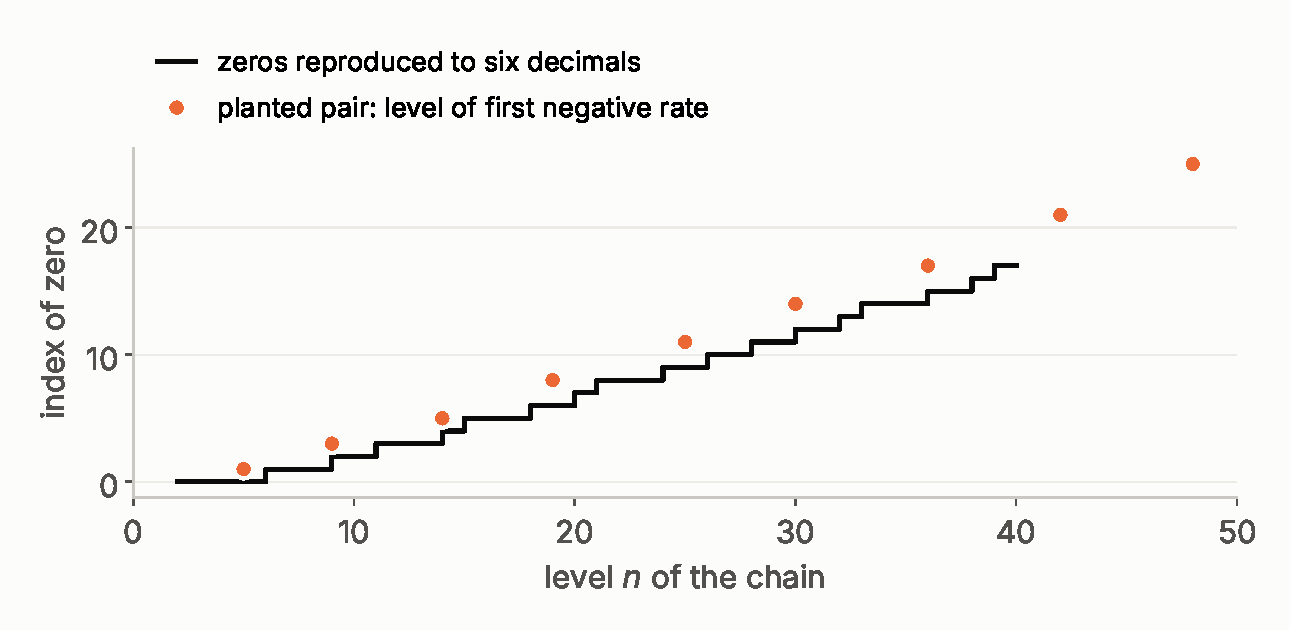
\includegraphics[width=0.9\textwidth]{fig/v3/bd_fig_resolution.pdf}
\caption{Zeros reproduced to six decimals by level (line), and the level at which a planted pair is detected (points).}\label{b:fig:res}
\end{figure}

\section{The chain at depth: a Gamma chain and an arithmetic fluctuation}

The moment route is too expensive to follow the coefficients far. To see their law at depth we use a second route, which starts from the zeros. It assumes the zeros in its range are real, as they are known to be, so positivity is automatic and is not being tested. What it gives is the size and shape of the coefficients.

\subsection{A second route and a cross check}

The measure $\nu$ is assembled from three pieces: the $6703$ zeros below height $7000$, located with the Riemann and Siegel formula to about $10^{-6}$; smooth zeros $\gamma_k^\Gamma$ up to index $30000$, defined by
\begin{equation}\label{b:eq:smooth}
\vartheta(\gamma_k^\Gamma)=\pi(k-\tfrac32),\qquad
\vartheta(t)=\tfrac t2\log\tfrac{t}{2\pi}-\tfrac t2-\tfrac\pi8+\tfrac{1}{48t},
\end{equation}
so that the first smooth zero, $k=1$, is the zero $14.518$ of $\cos\vartheta$ at $\vartheta=-\pi/2$; and a lumped tail up to height $10^{13}$ that keeps the mass and mean of each geometric bin. Its total mass is $0.023104993116$, against $m_0=0.023104993115$. The Jacobi coefficients of $\nu$ and of $x\nu$ are computed by the Lanczos process with full reorthogonalisation in double precision, and the rates follow without subtraction from the two sets of parameters (computed).

The two routes share nothing: one uses only the moments of $\Phi$, the other only the zeros. They agree to $4\cdot10^{-11}$ for $j\le50$, to $4\cdot10^{-8}$ for $j\le200$ and to $9\cdot10^{-7}$ for $j\le467$ (computed; an independent rerun with $376$ true zeros and smooth zeros beyond agrees to $8\cdot10^{-8}$ at $j=1$ and $2\cdot10^{-5}$ at $j=240$, the difference being the truncation of the zeros). On the Lambert chain the second route reproduces Lambert's coefficients to $10^{-6}$ for $j\le799$.

\subsection{The Gamma chain}

Let $c_j^\Gamma$ be the rates of the chain built from the smooth zeros \eqref{b:eq:smooth} alone. This chain knows nothing of the primes. It is the chain of a function whose zeros are real by construction, the zeros of $\cos\vartheta$, and it depends only on the Gamma factor. Write
\[
c_j=c_j^\Gamma\,(1+\varepsilon_j).
\]

\begin{remark}[Computation: the fluctuation]\label{b:comp:deep}
For $1\le j\le2799$ (computed in double precision from the zeros):
\begin{enumerate}
\item $|\varepsilon_j|\le0.149$, the largest value occurring at $j=27$; for $j>1000$, $|\varepsilon_j|\le0.052$.
\item The mean of $\varepsilon_j$ is $0.0003$. Its standard deviation over windows of $160$ indices is $0.057$ near $j=100$, $0.031$ near $j=400$, $0.017$ near $j=1600$ and $0.013$ near $j=2600$, a decay close to $j^{-0.44}$.
\item The ratio $c_j\gamma_j^2$, averaged locally, is $1.49$ at $j=100$, $1.68$ at $j=400$, $1.77$ at $j=1000$ and $1.86$ at $j=2700$. The Gamma chain alone gives $1.50$, $1.78$ and $1.86$ at $j=100$, $1000$, $2700$.
\item The ratio of birth to death rate at level $n$ is $0.998$ at $n=100$ and $1.002$ at $n=1390$.
\end{enumerate}
\end{remark}
% UNVERIFIED: W3 V8 reproduced the Gamma chain to j=1399 only (c_j^Gamma at j=10, 30, 100, 300, 1000 agree with the draft to 6 to 7 digits); the depth 2799 table, the statistics of epsilon_j and the figures below were not rerun. The values 1.77 and 1.86 for the true chain and the Gamma chain values at j=1000, 2700 are the draft's.

\begin{figure}[ht]
\centering
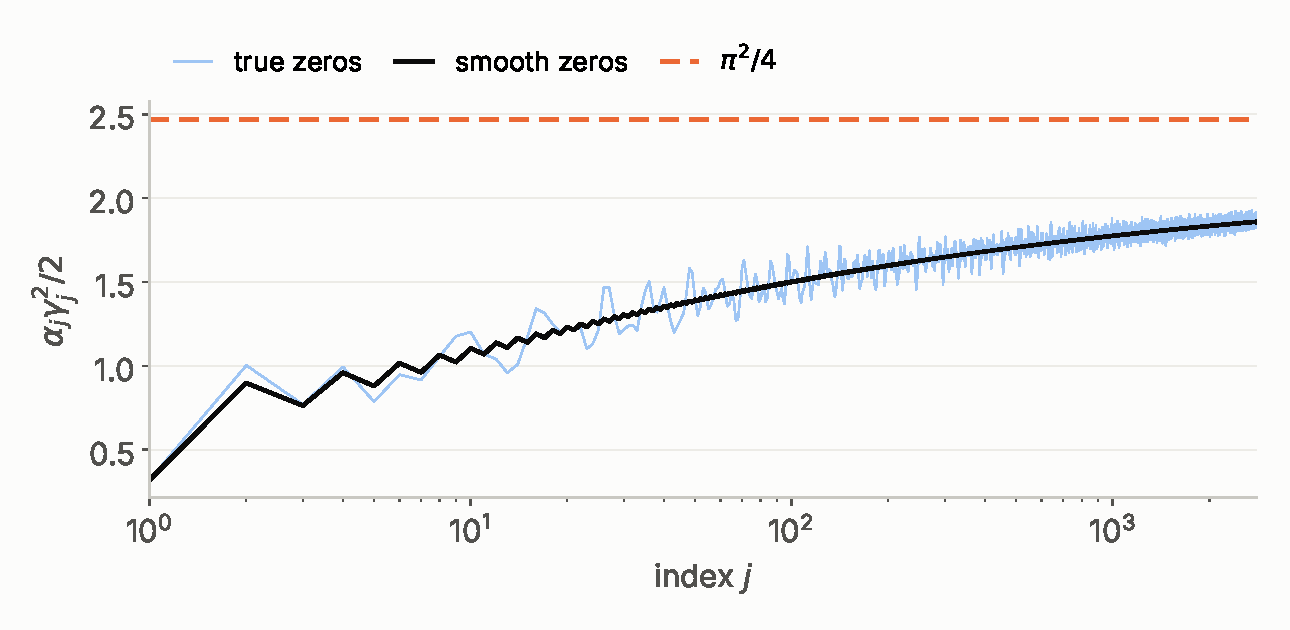
\includegraphics[width=0.95\textwidth]{fig/v3/bd_fig_deep_ratio.pdf}
\caption{The ratio $c_j\gamma_j^2$ to depth $2799$, for the true zeros and for the smooth zeros.}\label{b:fig:ratio}
\end{figure}

\begin{figure}[ht]
\centering
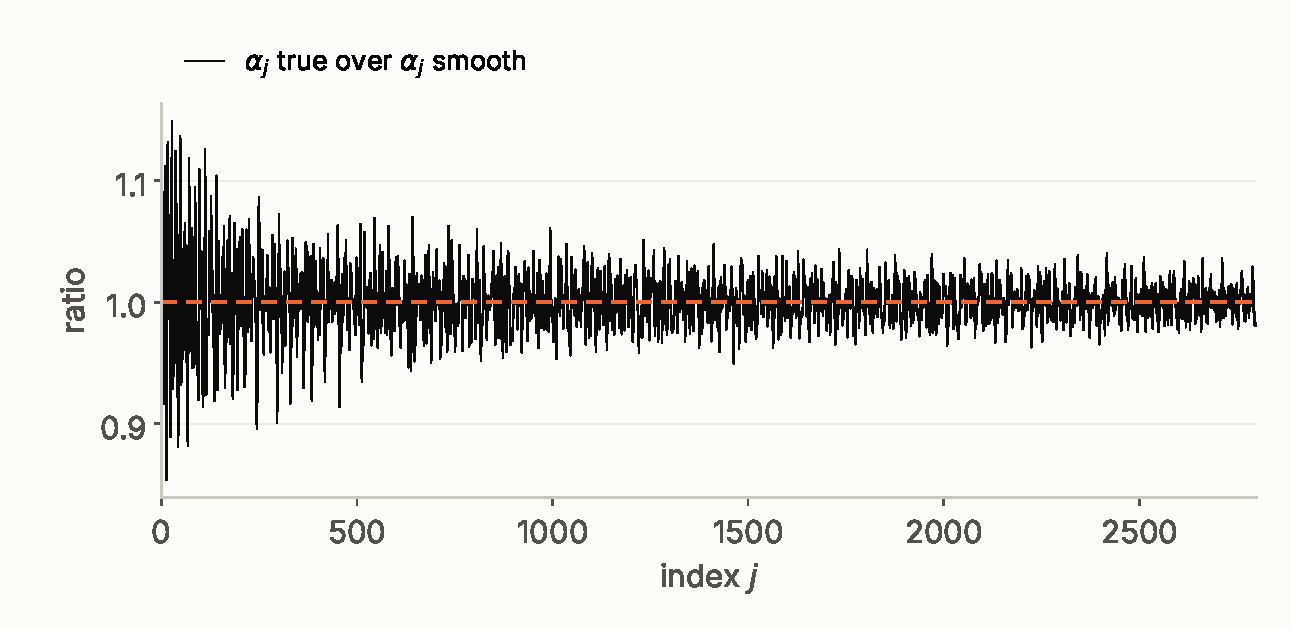
\includegraphics[width=0.95\textwidth]{fig/v3/bd_fig_arith.pdf}
\caption{The arithmetic factor $1+\varepsilon_j=c_j/c_j^\Gamma$.}\label{b:fig:arith}
\end{figure}
% The plotted values of these two figures were not rerun beyond j=1399 (W3 V8).

Fits of the form $A+B/\log$ to the ratio on $200\le j\le2700$ give $A=2.38$, $2.37$ and $2.60$ according as the logarithm is taken of $j$, of $\gamma_j/2\pi$ or of $\gamma_j$ (computed). The value $\pi^2/4=2.467$ of every Bessel model lies inside this range.

\begin{conjecture}\label{b:conj:law}
\begin{enumerate}
\item $c_j^\Gamma\gamma_j^2\to\pi^2/4$, at a logarithmic rate.
\item $\varepsilon_j\to0$.
\end{enumerate}
\end{conjecture}

Part 1 concerns the Gamma factor only. Section~\ref{b:sec:bs} derives it, heuristically and with its rate, from a semiclassical law. Part 2 implies that $c_j>0$ for all large $j$.

\subsection{What the decomposition means}

In this representation RH reads $\varepsilon_j>-1$ for every $j$. The computed fluctuation never exceeds $15$ per cent and shrinks with depth, so the margin is wide wherever we can see. Three cautions keep this in proportion.

\begin{enumerate}
\item The smallness of $\varepsilon_j$ was computed from real zeros. It is a consequence of their reality on the computed range, not evidence independent of it.
\item The chain is not stable under complex perturbations. In the toy model a pair at distance $0.01$ from the line turns a coefficient negative almost as early as a pair at distance $0.4$. A perturbation argument from the Gamma chain therefore cannot work in a norm that ignores the direction of the perturbation.
\item What the decomposition does supply is the correct statement to aim at. The primes enter the chain only through $\varepsilon_j$, and a proof must bound that single sequence from below by $-1$.
\end{enumerate}

\section{The Bohr and Sommerfeld law of the Gamma chain}\label{b:sec:bs}

The rates of the Gamma chain can be found in closed form to leading order. The argument is semiclassical and is not a proof. The same law, with the same constant $\frac74$, is stated as equation~\eqref{eq:ch21:ratelaw} of Volume II, with a comparison with the $1299$ certified rates of the note. What is added here is the Abel inversion written out, the split of the constant into birth and death levels, the generalisation to a conductor $q$, and the consequences.

\subsection{The zeros as eigenvalues}

Let $\tilde\nu$ be the symmetric measure on the line with mass $\frac12\gamma_k^{-2}$ at each of $\pm\gamma_k^{-1}$. Its orthonormal polynomials satisfy $y\,p_j=w_{j+1}p_{j+1}+w_jp_{j-1}$ with $w_j=\sqrt{c_j}$; this is the classical passage between a Stieltjes continued fraction and a symmetric Jacobi matrix. So the Jacobi matrix $W$ with zero diagonal and off diagonal entries $\sqrt{c_1},\sqrt{c_2},\dots$ has the eigenvalues $\pm1/\gamma_k$, $k=1,2,\dots$ Finding the chain from the zeros is an inverse spectral problem for $W$.

\subsection{The quantisation rule}

Suppose $w_n$ varies slowly with $n$. A solution of $w_{n+1}u_{n+1}+w_nu_{n-1}=\mu u_n$ oscillates where $2w_n>\mu$, with phase advancing by $\arccos(\mu/2w_n)$ per site, and decays beyond the turning point $n_*(\mu)$ where $2w_{n_*}=\mu$. The rule of Bohr and Sommerfeld gives the number of eigenvalues above $\mu$:
\begin{equation}\label{b:eq:BS}
N_W(\mu)=\frac1\pi\int_0^{n_*(\mu)}\arccos\frac{\mu}{2w(n)}\,dn+O(1).
\end{equation}
The turning point of the eigenvalue $\mu=1/\Gamma$ is the index at which $H_j=1/(2w_j)=\Gamma$. We call $H_j$ the turning height of coefficient $j$; it is $g_j$ of \eqref{eq:ch21:ratelaw}, and $c_j=1/(4H_j^2)$.

\begin{lemma}[Abel inversion]\label{b:lem:abel}
Let $f=2w$ be decreasing with inverse function $n(f)$. Then
\[
\frac1\pi\int_0^{n_*(\mu)}\arccos\frac{\mu}{f(n)}\,dn
=\frac1\pi\int_\mu^\infty n(f)\,\frac{\mu\,df}{f\sqrt{f^2-\mu^2}} .
\]
If $n(f)=\frac af\log\frac bf+c$ the right side equals $\frac{a}{\pi\mu}\bigl(\log\frac{2b}{\mu}-1\bigr)+\frac c2$.
\end{lemma}
\begin{proof}
Integrate by parts in the variable $f$, using $\frac{d}{df}\arccos(\mu/f)=\mu/(f\sqrt{f^2-\mu^2})$. For the second statement put $f=\mu/t$ and use $\int_0^1t(1-t^2)^{-1/2}dt=1$, $\int_0^1t\log t\,(1-t^2)^{-1/2}dt=\log2-1$ and $\int_\mu^\infty\mu\,df/(f\sqrt{f^2-\mu^2})=\frac\pi2$.
\end{proof}

The eigenvalues above $\mu$ correspond to the zeros below height $\Gamma=1/\mu$, and for the smooth zeros \eqref{b:eq:smooth} their number is $\vartheta(\Gamma)/\pi+\frac32=\frac{\Gamma}{2\pi}(\log\frac{\Gamma}{2\pi}-1)+O(1)$. Equating this with \eqref{b:eq:BS} through Lemma~\ref{b:lem:abel} forces $a=\frac12$ and $b=1/(4\pi)$, that is $n=\frac{H}{2}\log\frac{H}{4\pi}$ with $H=1/f$.

\begin{conjecture}[Bohr and Sommerfeld law]\label{b:conj:bs}\label{b:prop:bs}\label{b:prop:bs2}
The Gamma chain of a function with conductor $q$ whose smooth zero count $N(\gamma)=\frac\gamma{2\pi}\log\frac{q\gamma}{2\pi e}+C+o(1)$ is normalised by $N(\gamma_k)=k-\frac12$ has rates
\[
c_j^\Gamma=\frac1{4H_j^2},\qquad \frac{H_j}2\log\frac{qH_j}{4\pi}=j-2C+O\Bigl(\frac1{\log H_j}\Bigr).
\]
For $\xi$, $q=1$ and $2C=\frac74$, which is \eqref{eq:ch21:ratelaw}.
\end{conjecture}

The same argument applied to a Bessel chain, where the count is linear, gives $c_j=1/(4(j+c)^2)$, in agreement with the exact coefficients of Proposition~\ref{b:prop:bessel}. The logarithm in the law is the logarithm in the density of the zeros. The derivation is heuristic: Lemma~\ref{b:lem:abel} is exact, but the rule \eqref{b:eq:BS} is used in the inverse direction and assumes that the coefficients vary regularly. Section~\ref{b:sec:c0} gives the constant.

\begin{table}[ht]
\centering\small
\begin{tabular}{@{}rccr@{}}
\toprule
$j$ & Gamma chain $c_j^\Gamma$ & law with constant $2$ & relative error\\
\midrule
10 & $4.3768\cdot10^{-4}$ & $4.2390\cdot10^{-4}$ & $-0.0315$\\
30 & $1.2770\cdot10^{-4}$ & $1.2692\cdot10^{-4}$ & $-0.0061$\\
100 & $2.6996\cdot10^{-5}$ & $2.6978\cdot10^{-5}$ & $-0.0006$\\
300 & $5.6038\cdot10^{-6}$ & $5.6041\cdot10^{-6}$ & $0.0001$\\
1000 & $8.809\cdot10^{-7}$ & $8.810\cdot10^{-7}$ & $0.0001$\\
\bottomrule
\end{tabular}
\caption{The law with constant $2$ against the computed Gamma chain, at even $j$ (death rates). On $100\le j<1000$ the largest relative error over all $j$ is $3.2\cdot10^{-3}$, at $j=101$; on $j\ge1000$ it is of the order $4\cdot10^{-4}$ (computed).}\label{b:tab:law}
\end{table}
% UNVERIFIED: the 1000 row and the bound for j>=1000: W3 V8 gives 1.761818e-6 (alpha) for j=1000, 9e-6 relative to the draft, and 3.8e-4 on 1001 to 1399; the draft's 3.7e-4 extends to 2799. The row j=2799 was dropped.

The table lists only even $j$, and the accuracy depends on the parity. With constant $2$ the relative error at the odd (birth) indices $j=101$, $201$, $301$ is $3.2\cdot10^{-3}$, $1.7\cdot10^{-3}$ and $1.2\cdot10^{-3}$, against $6\cdot10^{-4}$, $4\cdot10^{-5}$ and $7\cdot10^{-5}$ at the even neighbours. With the constant $\frac74$ of the next subsection the pattern reverses: about $2\cdot10^{-4}$ at odd $j$ and up to $4.1\cdot10^{-3}$ at even $j$ (computed). So the law holds for the means of the birth and death rates, to a few parts in a thousand, not to two parts in ten thousand.

\begin{corollary}\label{b:cor:limit}
Assume the law of Conjecture~\ref{b:conj:bs} for $\xi$ and put $\rho_j=\gamma_j/(\pi H_j)$ and $L_j=\log(H_j/2)$. Then
\[
c_j^\Gamma\gamma_j^2=\frac{\pi^2}{4}\,\rho_j^2,\qquad
\rho_j\bigl(L_j+\log\rho_j-1\bigr)=L_j-\log2\pi+o(1),
\]
so the ratio tends to $\pi^2/4$ and $1-\rho_j\sim(\log2\pi-1)/L_j$.
\end{corollary}
\begin{proof}
$\gamma_j$ satisfies $\frac{\gamma}{2\pi}\log\frac{\gamma}{2\pi e}=j+O(\log j)$ and $H_j$ satisfies $\frac H2\log\frac H{4\pi}=j+O(1)$. Substitute $\gamma=\pi\rho H$.
\end{proof}

At $j=100$, $1000$, $2700$ the computed $\rho_j$ are $0.781$, $0.848$, $0.867$, giving $\frac{\pi^2}{4}\rho_j^2=1.50$, $1.78$, $1.86$, the values of Computation~\ref{b:comp:deep}. The slow rise seen in Figure~\ref{b:fig:ratio} is the factor $\rho_j^2$, and its limit is $\pi^2/4$ (heuristic, from the law). % UNVERIFIED: only rho_100 = 0.781 was recomputed (U06); the values at 1000 and 2700 are the draft's.

\begin{remark}[Resolution, heuristic]\label{b:cor:res}
If the law holds, the turning point of the eigenvalue $1/\Gamma$ is at the index $j$ with $H_j=\Gamma$. So the first $j$ coefficients determine the zeros up to height about $H_j$, and the fraction of zeros resolved per coefficient tends to $1/\pi$. For $j=467$ this gives height $295$; the level $234$ chain reproduced the zeros to six decimals up to height $279$. The rule is consistent with the detection level of the toy model: a pair above the $k$th zero is seen once $H_j$ passes its height.
\end{remark}

\subsection{The constant: $2C$ is the constant term of the zero count}\label{b:sec:c0}

Write the smooth zero count of a Gamma chain as in Conjecture~\ref{b:conj:bs}. The Abel inversion of Lemma~\ref{b:lem:abel} reads
\begin{equation}\label{b:eq:abelj}
j(H)=2H\int_0^H\frac{dN(\gamma)}{\sqrt{H^2-\gamma^2}},\qquad c_j=\frac{1}{4H_j^2}.
\end{equation}
The logarithmic density gives $\frac H2\log(qH/4\pi)$, which is exact. The constant term enters as a jump of size $C$ at $\gamma=0$ in the continuation of the smooth count, and the kernel $2H/\sqrt{H^2-\gamma^2}$ equals $2$ there. The prediction is therefore
\begin{equation}\label{b:eq:c0}
\frac{H_j}2\log\frac{qH_j}{4\pi}=j-2C+O\Bigl(\frac{1}{\log H_j}\Bigr).
\end{equation}

The Bessel chain tests the mechanism exactly. The zeros $j_{\nu,k}\approx\pi(k+\frac\nu2-\frac14)$ give $N(\gamma)=\gamma/\pi-\frac\nu2-\frac14$, so \eqref{b:eq:abelj} gives $j(H)=H-\nu-\frac12$. The exact coefficients have $H_j=\sqrt{(\nu+j)(\nu+j+1)}=\nu+j+\frac12+O(1/j)$, so the law holds with no further constant.

For $\xi$, $N=\vartheta/\pi+1$ and $\vartheta(t)=\frac t2\log\frac{t}{2\pi e}-\frac\pi8+O(1/t)$, so $C=\frac78$ and $2C=\frac74$. For a Dirichlet $L$ function of conductor $q$ with $\Gamma(\frac{s+a'}{2})$, $a'\in\{0,1\}$, the smooth zeros of our Gamma chains satisfy $\vartheta_\chi(\gamma_k)/\pi=k-\frac12$ (the constant term of $\vartheta_\chi$ being $-\pi/8$ for the even character), and Stirling's formula gives $C=(a-\frac12)/2$ with $a=\frac14$ (even) or $\frac34$ (odd), so $2C=-\frac14$ or $\frac14$.

\begin{remark}[Computation: the constant]\label{b:comp:c0}
Fit $j-\frac{H_j}2\log(qH_j/4\pi)$ by $c_\infty+B/L+B_2/L^2$, $L=\log(qH_j/4\pi)$, separately on birth levels ($j$ odd) and death levels ($j$ even), for three Gamma chains: $\xi$ ($q=1$), $L(s,\chi_{12})$ ($q=12$, even, $60\le j\le560$) and conductor $5$, odd ($40\le j\le300$), the Gamma chain of the Davenport and Heilbronn function.
\begin{center}\small
\begin{tabular}{@{}lcccc@{}}
\toprule
chain & $2C$ & $c_\infty$ birth & $c_\infty$ death & $B$ birth, death\\
\midrule
$\xi$ ($60\le j\le1399$) & $1.7500$ & $1.7514$ & $1.7747$ & $0.03$, $0.71$\\
$L(s,\chi_{12})$ & $-0.2500$ & $-0.2426$ & $-0.2399$ & $-0.08$, $0.72$\\
cond. $5$, odd & $0.2500$ & $0.2595$ & $0.2669$ & $-0.04$, $0.61$\\
\bottomrule
\end{tabular}
\end{center}
The residual of the fit for $\xi$ is $6\cdot10^{-4}$ (the fit on $60\le j\le1500$ gave $1.7478$ and $1.7772$). Birth levels carry almost no $1/L$ term; death levels carry $B\approx0.6$ to $0.7$ and reach the same limit more slowly. The fitted constants lie within $0.03$ of $2C$ (computed).
\end{remark}
% UNVERIFIED: the rows for L(s,chi_12) and conductor 5 and the residuals 1e-4, 2e-5 were not rerun; the xi row is the W3 V10 refit (c_inf 1.7514, 1.7747, B 0.030, 0.706).

\begin{figure}[ht]\centering
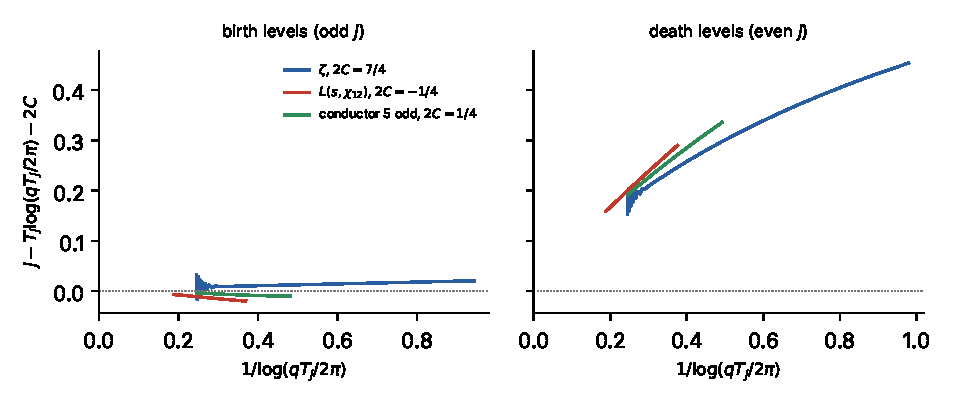
\includegraphics[width=\textwidth]{fig/v3/bd_fig_law.pdf}
\caption{$j-\frac{H_j}2\log(qH_j/4\pi)-2C$ against $1/\log(qH_j/4\pi)$ for three Gamma chains. Birth levels sit on the prediction; death levels approach it linearly in $1/\log H_j$. The wiggle in the $\xi$ curve near $0.25$ is the edge of the lumped tail.}
\end{figure}
% The figure was drawn from the fit on 60 <= j <= 1500; W3 V10 reproduced the same picture with fits 0.003 different.

The law now predicts where a zero off the line is seen. For the Davenport and Heilbronn zeros at heights $85.70$ and $114.16$, \eqref{b:eq:c0} with $H=\gamma$, $q=5$, $2C=\frac14$ gives $j=151.48$ and $218.08$, against the failures at $148$ to $150$ and $217$ to $219$ of Computation~\ref{b:comp:dh}. The first zero, farther from the line ($\beta-\frac12=0.31$), is seen about two indices early.

\begin{remark}[What is proved and what is not]\label{b:rem:bsstatus}
Exact: the Abel transforms, Lemma~\ref{b:lem:abel} and \eqref{b:eq:abelj}, and the Bessel case, where the coefficients are known in closed form. Heuristic: the semiclassical count \eqref{b:eq:BS} in the inverse direction, and with it the value $2C$, which the computation confirms to about $0.03$ on three chains. Note that the quantisation integral by itself does not give the constant: for the law chain with constant $\frac74$ an independent computation finds the arccos sum $\frac1\pi\sum_j\arccos(\mu/2w_j)$ smaller than the smooth count by about $\frac14$ in the limit, a term of Maslov type that the Abel kernel does not contain. So $2C=\frac74$ rests on the chain computations and on the integer eigenvalue count, not on the lemma. Unexplained: the death level coefficient $B$. A proof of the leading order should come from a Tauberian theorem for Krein strings of the kind due to Kasahara, which links regular variation of the spectral function to regular variation of the string; we have not checked its hypotheses for the discrete strings here. A proof needs two steps: the direct statement, that a Jacobi matrix with weights given by the law has the stated eigenvalue count, and a uniqueness or stability argument for the inverse problem with the weights $\gamma_k^{-2}$. Neither is supplied here. % TODO: Kasahara has no reference in the bibliography; add one or cut the name (review minor).
\end{remark}

With the law, the statement of RH in this chapter takes its final form, conditional on the law. The chain of the zeros has coefficients
\[
c_j=\frac{1+\varepsilon_j}{4\,H_j^2}\,(1+o(1)),
\]
where $H_j$ is explicit and involves only the Gamma factor, and RH is the inequality $\varepsilon_j>-1$.

\section{The arithmetic fluctuation: what the primes explain}\label{b:sec:prime}

The natural hope is a formula for $\varepsilon_j$ as a sum over primes, which could then be bounded below. The semiclassical argument produces a candidate at once. The computation does not support it, and we record both. Everything in this section is heuristic or computed.

\subsection{The candidate}

Lemma~\ref{b:lem:abel} can be inverted for any counting function $N$. In terms of the turning height $H$ it reads
\begin{equation}\label{b:eq:inv}
j(H)=\frac2H\int_0^H\frac{\Gamma\,d[\Gamma N(\Gamma)]}{\sqrt{H^2-\Gamma^2}} ,
\end{equation}
and for the counting function of a set of zeros, $j(H)=2H\sum_{\gamma<H}(H^2-\gamma^2)^{-1/2}$. A perturbation $\delta N(\Gamma)=A\sin(\omega\Gamma)$ gives
\[
\delta j(H)=A\,\pi\,\omega H\,J_0(\omega H),
\]
by the integrals $\int_0^{\pi/2}\sin\theta\sin(z\sin\theta)\,d\theta=\frac\pi2J_1(z)$ and $\int_0^{\pi/2}\sin^2\theta\cos(z\sin\theta)\,d\theta=\allowbreak\frac\pi2(J_0(z)-J_1(z)/z)$. Inserting the formal expansion $S(t)=\allowbreak-\frac1\pi\allowbreak\sum_n\Lambda(n)n^{-1/2}\allowbreak\sin(t\log n)/\log n$ of the fluctuation of the zero count, and $\varepsilon_j\approx\allowbreak4\,\delta j\allowbreak/\allowbreak(H_j(\log(H_j/4\pi)+1))$ from the law,
\begin{equation}\label{b:eq:cand}
\varepsilon_j\ \overset{?}{\approx}\
-\frac{4}{\log(H_j/4\pi)+1}\sum_{n\ge2}\frac{\Lambda(n)}{\sqrt n}\,
J_0\bigl(H_j\log n\bigr).
\end{equation}
The candidate has the right shape in two respects: its terms oscillate in the turning height $H_j$ with the frequencies $\log n$, and their amplitude decays like $H_j^{-1/2}$, close to the observed $j^{-0.44}$.

\subsection{The test}

\begin{remark}[Computation: the candidate against the chain]\label{b:comp:prime}
For $100<j\le2799$ (computed):
\begin{enumerate}
\item The zero form of \eqref{b:eq:inv}, regularised by a small imaginary part of $H$, reproduces the Gamma chain (residual $0.4$ in the index for regularisation $1$) but not the true chain: the residual is as large as the fluctuation itself for every regularisation tried.
\item With the staircase replaced by a smooth interpolant through the zeros, the predicted and observed shifts of the index have correlation $-0.04$.
\item A regression of $\varepsilon_j$ on the terms of \eqref{b:eq:cand} with free amplitude and phase for each $n$ finds one clear line, at $n=2$: amplitude $0.64$ of the candidate value, phase shifted by $-0.85$ radians. For $n=3,4,5,7,8,9,11$ the fitted amplitudes lie between $0.003$ and $0.046$, no larger than those of the controls $n=6,10,12,14,15$, which lie between $0.032$ and $0.057$.
\item The terms $n=2,3$ explain $6$ per cent of the variance of $\varepsilon_j$.
\end{enumerate}
\end{remark}
% UNVERIFIED: the statistics of epsilon_j, regressions, periodograms and the clock fits of this section were not rerun (W3 NOT DONE list).

So \eqref{b:eq:cand} is not the formula. The prime $2$ is the strongest line in the chain, at frequency $\log2$ in the turning height. The lines at the other small integers appear only after the lattice dispersion is taken into account, below.

\subsection{Where the fluctuation comes from}

\begin{remark}[Computation: a local regression]\label{b:comp:local}
(Computed.)
\begin{enumerate}
\item The fluctuations of the birth and death rate at the same level have correlation $0.65$. Between consecutive levels the correlation of the product $c_{2n-1}c_{2n}$ is $0.24$.
\item A linear regression of $\varepsilon_j\sqrt{H_j}$ on the displacements of the $25$ zeros nearest the turning height explains $21$ per cent of the variance, and between $23$ and $29$ per cent when the fit is allowed to depend on where the turning height falls between two zeros.
\end{enumerate}
\end{remark}

This regression suggests that the fluctuation is local, but the suggestion is superseded. With the exact Jacobian of the rates with respect to the zeros (Theorem~\ref{pp:thm:lr}, Chapter~\ref{ch:progress}), a three point rule along the straight path from the smooth zeros to the true zeros reproduces $\varepsilon_j$ to a coefficient of determination of $0.9993$ through $j=1999$. So the fluctuation is a smooth and only mildly nonlinear function of the displacements, and the regression above failed because the response is not local: it extends over about a hundred zeros, almost all above the turning height. The index spacing in the turning height is about one third of the mean spacing of the zeros, so the chain reads the zeros nearly one at a time as the turning height passes them, but it does so through a long kernel. For the programme this is a negative result with a definite content: a lower bound $\varepsilon_j>-1$ cannot be read off from a convergent prime sum of the form \eqref{b:eq:cand}.

\subsection{Spectral lines and a lattice dispersion}

\begin{remark}[Computation: spectral lines]\label{b:comp:lines}
Let $h_j=H_{j+1}-H_j$ be the step of the turning height. The periodogram of $\varepsilon_j\sqrt{H_j}$ in the variable $H_j$, for $150<j\le 2799$, has lines close to $\log n$ for $n=2,\dots,10$ and $n=12$, with peak power over median power $311$, $197$, $128$, $81$, $61$, $38$, $32$, $19$, $14$ for $n=2,\dots,10$ (computed).
\begin{enumerate}
\item The lines sit above $\log n$. With $w=\log n$ the peak frequency is $w+c\,w^{3}$ and $c=0.0041$ to within five per cent for $3\le n\le 8$.
\item The constant $c$ falls with depth: $0.0051$, $0.0040$, $0.0037$ on $150<j\le900$, $900<j\le1800$, $1800<j\le2799$, where the mean of $h_j^{2}/24$ is $0.0097$, $0.0068$, $0.0057$. A fit with phase $wH_j+\kappa w^{3}\sum_{i\le j}h_i^{3}$ gives $\kappa=0.036$, against $1/24=0.042$ for the dispersion $(2/h)\arcsin(wh/2)$ of a lattice of step $h$.
\item Lines appear at $n=6$, $10$ and $12$ as well as at prime powers, and the peak amplitude falls smoothly with $n$, between $n^{-1/2}$ and $n^{-1}$.
\item A sum over $2\le n\le 30$ with weights $n^{-\sigma}$ and one common phase explains $16$ per cent of the variance at best. With a free amplitude and phase for each $n\le 40$ the lines explain $22$ per cent in sample, and a fit on the first half of the levels explains nothing on the second half.
\end{enumerate}
\end{remark}

The clock of the candidate \eqref{b:eq:cand} was therefore wrong in one respect: the chain is a lattice in $j$, and a wave of frequency $w$ in height is seen with the lattice dispersion and not with frequency $w$. This is why the fixed frequency regression of Computation~\ref{b:comp:prime} found only the line at $n=2$. The correction does not rescue the formula. The lines carry about one fifth of the fluctuation, their phases are not stable across the range, and their presence at composite $n$ with smooth amplitudes is not the signature of $\zeta'/\zeta$. The peak search in item 3 is also a maximum over a window, so the weaker lines should be read with care.

\subsection{A common dispersion clock and a Dirichlet series model}

The lines of Computation~\ref{b:comp:lines} are coherent. Demodulating each line in windows of width $120$ in $H$ shows a phase that drifts smoothly across the whole range, and the total drift divided by $w^3$ is nearly the same for every line: $3.6$, $3.9$, $4.0$, $4.1$ for $n=2,3,4,5$. So a single clock serves all frequencies. Write $h(H)=2/(\log(H/4\pi)+1)$ for the step of the turning height implied by the law and $I(H)=\int^{H}h(x)^2\,dx$.

\begin{remark}[Computation: a common clock]\label{b:comp:clock}
Fit on the levels with $H<726$ (the first half) the five parameter model
\[
\varepsilon_j\sqrt{H_j}\approx \re\Bigl[A\,e^{i\phi}\sum_{n=2}^{40}n^{-\sigma}
\exp\bigl\{i\bigl(H_j\log n+(g_0+\beta I(H_j))\log^3 n\bigr)\bigr\}\Bigr],
\]
and test it on the levels with $H>726$ (computed).
\begin{enumerate}
\item The fit gives $\sigma=1.28$, $\beta=0.023$, and explains $44$ per cent of the variance on the first half and $25$ to $27$ per cent on the unseen second half. On all levels it explains $38$ per cent.
\item Free amplitudes and phases for each $n\le12$, with the same clock, explain $56$ per cent in sample and $13$ per cent out of sample: the common phase of the series is not an artefact of overfitting.
\item The amplitudes of the lines at $\log(pq)$ and $\log(q/p)$ are about twice the product of the amplitudes at $\log p$ and $\log q$, for ten pairs, as second order mixing would give.
\item The weights cannot be identified. With the same clock, $\zeta$, $\zeta'/\zeta$ and $\log\zeta$ weights predict $27$, $28$ and $27$ per cent of the second half; $\zeta^2$ and Liouville weights $20$ and $21$; $1/\zeta$ weights $14$. The fit is carried by the lines with $n\le5$.
\item The residual has lag one autocorrelation $0.53$, sits in the band of frequencies $0.6$ to $4.1$, and has no correlation above $0.09$ with the normalised gap at $aH$, or the distance to the nearest zero, for $a$ from $1/4$ to $2$. The earlier correlation $-0.17$ with $|Z(H_j)|$ is carried by the lines.
\end{enumerate}
\end{remark}

The constant $\beta=0.023$ is about half the value $1/24$ for an ideal lattice, and a $\log^3 n$ phase is what an Airy kernel at a turning point produces, so the clock may be the Airy layer of the orthogonal polynomials at height $H_j$. This is an interpretation, not a derivation.

What the model would mean, if it held exactly. A series with $\sigma>1$ is absolutely convergent and bounded by $|A|(\zeta(\sigma)-1)$, where the amplitude $|A|$ is not reported, so no numerical bound follows. Then $|\varepsilon_j|\le C_A H_j^{-1/2}$ for a constant $C_A$, and $\varepsilon_j>-1$ would follow for every level with $H_j$ large enough, leaving a finite check. The decay of the spread of $\varepsilon_j$ like $j^{-0.44}$ found in Computation~\ref{b:comp:deep} is consistent with the factor $H_j^{-1/2}$. But the model explains well under half of the variance, and a pair of zeros off the line would add a localised negative excursion that no absolutely convergent series can produce. The precise target is therefore the following.

\begin{conjecture}\label{b:conj:ap}
There is a function $F$, almost periodic in the sense of Besicovitch with frequencies in the additive group generated by $\{\log p\}$ and dispersed by a clock $\beta I(H)$, such that $\varepsilon_j\sqrt{H_j}=F(H_j)+o(1)$ and $\sup|F|<\infty$.
\end{conjecture}

A bounded $F$ gives $\varepsilon_j\to0$ and hence $c_j>0$ for all but finitely many $j$; the remaining levels are a finite computation. It is not known to follow from RH, and it is not proved here. It is, however, testable level by level, and it separates the arithmetic part of the chain, which the primes appear to control, from the part that must carry any violation.

\begin{figure}[ht]\centering
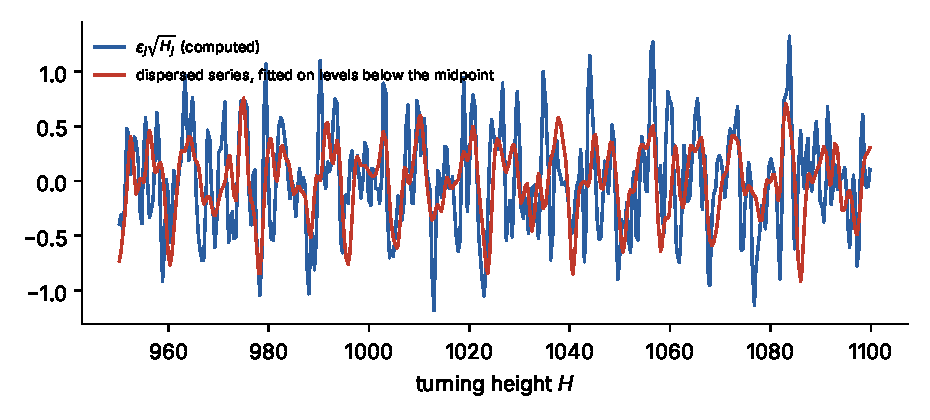
\includegraphics[width=\textwidth]{fig/v3/bd_fig_oos.pdf}
\caption{The fluctuation $\varepsilon_j\sqrt{H_j}$ and the dispersed series of Computation~\ref{b:comp:clock}, fitted on levels with $H<726$ and shown on $950<H<1100$.}
\end{figure}

\section{A second L function: the Dedekind eta function}\label{b:sec:eta}

For the even primitive character $\chi_{12}$ ($\chi_{12}(n)=1$ for $n\equiv\pm1$, $-1$ for $n\equiv\pm5 \bmod 12$) the theta function is the eta function itself,
\[
\theta(x)=\sum_{n\ge1}\chi_{12}(n)e^{-\pi n^2x/12}=\eta(ix),\qquad \eta(i/x)=\sqrt{x}\,\eta(ix),
\]
so $f(y)=e^{y/2}\eta(ie^{2y})$ is even and $\Lambda(\tfrac12+v,\chi_{12})=(12/\pi)^{(1/2+v)/2}\Gamma(\tfrac{1/2+v}{2})L(\tfrac12+v,\chi_{12})$ is a constant times $\int_0^\infty f(y)\cosh(vy)\,dy$. The chain of $G_\chi(u)=\Lambda(\frac12+\sqrt u,\chi_{12})/\Lambda(\frac12,\chi_{12})$ is therefore defined by the eta function alone.

\begin{remark}[Computation: the chain of $\chi_{12}$]\label{b:comp:eta}
\begin{enumerate}
\item The identities above hold numerically to working precision, and $m_0=\Lambda''(\tfrac12)/(2\Lambda(\tfrac12))=0.1664618041$ from the kernel agrees with $\sum_\gamma \gamma^{-2}$ from the zeros, to $10^{-7}$ (the size of the smooth tail correction). $L(\tfrac12,\chi_{12})=0.4985570025$.
\item The first zeros are $3.80462763$, $6.69222332$, $8.89059296$, $11.18839275$, $12.96617881$. All zeros below height $100$ were found, with $k-\vartheta_\chi(\gamma_k)/\pi$ between $0.17$ and $0.84$.
\item The moment route from $\eta$ alone at $1500$ digits gives $c_j>0$ for every $j\le300$, with minimum about $1.5\cdot10^{-5}$ at $j=300$. A run at $1800$ and $2100$ digits, agreeing to $10^{-10}$ through $j=533$, reported $c_j>0$ for every $j\le533$ with minimum $5.9\cdot10^{-6}$. The cost is close to that for $\xi$.
\item The zeros route with zeros to height $100$ and smooth zeros beyond agrees with the moment route to $3\cdot10^{-6}$ for $j\le10$ and $5\cdot10^{-4}$ for $j\le100$.
\end{enumerate}
\end{remark}
% UNVERIFIED: W3 V9 confirmed items 1 and 2 (the draft's zeros 2 and 4 were wrong in the sixth decimal and are corrected here) and positivity to j=300 at one precision only; the run to 533 and item 4 were not rerun. All values are floating point or mpmath, not ball arithmetic.

Positivity of the first $J$ rates verifies no zero of $L(s,\chi_{12})$: the criterion needs every $j$, and no argument we know turns finitely many positive rates into reality of the zeros below a height. The book's Proposition~\ref{prop:ch21:verhankel} goes the other way: verified zeros imply positivity up to order about $5\sqrt M$, and it has a ceiling of order $\sqrt M$. The value of the computation is that the chain comes from the modular form without the zeros. A sharp test of Conjecture~\ref{b:conj:ap} is open: since $\chi_{12}(2)=\chi_{12}(3)=0$, an arithmetic fluctuation built from the coefficients of $L(s,\chi_{12})$ must lose the lines at $\log2$ and $\log3$ that dominate the $\zeta$ case. % TODO: the named computations (b:comp:etalines, drifts, R^2) lack % UNVERIFIED marks, W3 did not rerun them.

\begin{remark}[Computation: lines of $\chi_{12}$]\label{b:comp:etalines}
Compare the computed chain for $L(s,\chi_{12})$ with its own Gamma chain (smooth zeros $\vartheta_\chi(\gamma)/\pi=k-\frac12$, conductor $12$), so that $\varepsilon_j$ is obtained from $\eta$ without any zeros, for $61\le j\le533$ (turning heights about $35$ to $203$). Then $\max|\varepsilon_j|=0.096$. The periodogram of $\varepsilon_j\sqrt{H_j}$, as peak over median power in a window at $\log n$, gives for $n=2,3,4,6,8,9,10$, where $\chi_{12}(n)=0$, the values $1.7$, $1.1$, $1.4$, $2.1$, $1.4$, $1.0$, $1.9$: no lines. For $n=5,7,11,13$, where $\chi_{12}(n)\ne0$, it gives $10.3$, $8.0$, $5.6$, $5.1$. For $\zeta$ over the same heights the lines at $\log2$ and $\log3$ are the strongest, $8.9$ and $5.5$. (The value $5.5$ at $n=12$ is the line at $\log13$ inside the search window.)
\end{remark}

So the arithmetic fluctuation is built from the Dirichlet coefficients of the $L$ function itself. This is the strongest evidence so far for Conjecture~\ref{b:conj:ap}, and it is obtained from the modular form alone. It is evidence on one function over a short range, and the lines at $n=5,7,11,13$ are peaks over a window, with the caution already given.

\section{Calibration: a function with zeros off the line}\label{b:sec:dh}

The Davenport and Heilbronn function $f(s)=\sum a_nn^{-s}$, with $a_n=1,\kappa,-\kappa,-1,0$ for $n\equiv1,2,3,4,0 \bmod 5$ and $\kappa=(\sqrt{10-2\sqrt5}-2)/(\sqrt5-1)$ \cite{DH36}, satisfies $\Lambda(s)=\Lambda(1-s)$ for $\Lambda(s)=(5/\pi)^{(s+1)/2}\Gamma(\frac{s+1}{2})f(s)$ but has zeros off the critical line. Its theta function $\theta(x)=\sum na_ne^{-\pi n^2x/5}$ satisfies $\theta(1/x)=x^{3/2}\theta(x)$, so $K(y)=e^{3y/2}\theta(e^{2y})$ is even and the chain is defined exactly as for $\xi$. The first failure of the test, $c_{148}<0$, is in Section~\ref{sec:ch21:hankel}; what follows adds the second failure and the pattern.

\begin{remark}[Computation: the Davenport and Heilbronn chain]\label{b:comp:dh}
\begin{enumerate}
\item The transformation holds to working precision, and the kernel reproduces $\Lambda(\frac12+v)/\Lambda(\frac12)$. The first zeros off the line are $0.808517182+85.699348485i$ and $0.650830081+114.163342731i$ \cite{Spira94,BSO07}.
\item Kernel runs at $1100$ and $1400$ digits agree to thirty printed digits. Through $j=262$ exactly four rates are negative: $c_{148}=-8.9\cdot10^{-6}$, $c_{150}=-3.6\cdot10^{-4}$, $c_{217}=-4.0\cdot10^{-6}$, $c_{219}=-2.6\cdot10^{-4}$, and the neighbours $c_{149}$ and $c_{218}$ are positive (computed; a run to $j=319$ at $1000$ and $1250$ digits reported no others).
\item Against the Gamma chain of conductor $5$, away from the failures $|\varepsilon_j|\le0.165$, with median $0.034$. At the failures $\varepsilon_j=-1.25,+15.3,-11.5$ for $j=148,149,150$ and $-1.21,+18.4,-14.6$ for $j=217,218,219$.
\item The turning height $H_j$ of the Gamma chain reaches $85.70$ at $j=152$ and $114.16$ at $j=218$. The law with $q=5$, $2C=\frac14$ puts the turning levels at $151.48$ and $218.08$.
\end{enumerate}
\end{remark}
% UNVERIFIED: W3 V9 confirmed the four negative rates (halved here), no others through j=262 and the turning levels 151.48, 218.08; the epsilon values and bounds of item 3 and the zeros of item 1 beyond the draft's own values were not rerun.

\begin{figure}[ht]\centering
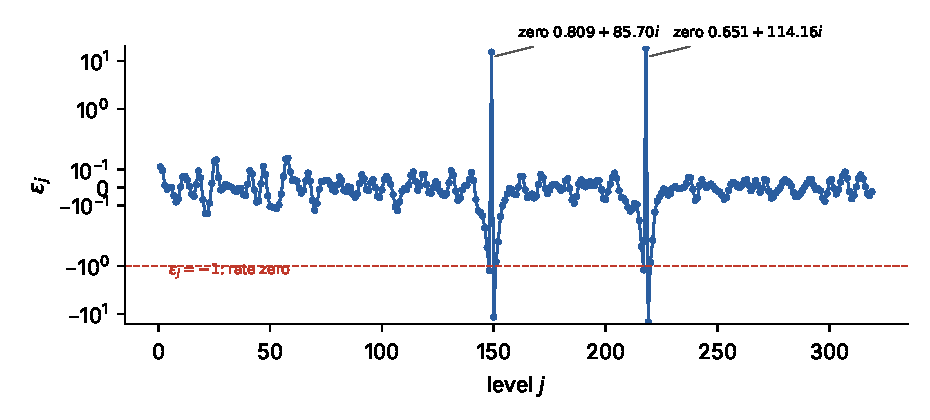
\includegraphics[width=\textwidth]{fig/v3/bd_fig_dh.pdf}
\caption{The fluctuation $\varepsilon_j$ of the Davenport and Heilbronn chain, symmetric log scale. Each zero off the line produces one localised triplet crossing $\varepsilon_j=-1$ at the level where the turning height reaches its ordinate.}
\end{figure}

Three facts are worth recording. First, the chain detects zeros off the line, as Grommer's theorem guarantees, and it does so sharply: a negative rate appears in a window of three levels. Second, the level is predicted in advance by the turning height of the Gamma chain, to within four levels. Third, each of the two pairs of zeros off the line costs exactly two negative rates, which is consistent with the Chebotarev count of negative terms of $D_{n-1}D_n$; this is two instances, not a law of the computation, and the general statement is Theorem~\ref{thm:ch12:inertia}. The size of the failure is not monotone in $\beta-\frac12$: the zero nearer the line gives the larger excursion, so the depth reflects where the level grid falls, not the distance from the line. Finally, the fluctuation away from the failures is of the same size as for $\zeta$ and $\chi_{12}$: there is a gap between about $0.17$ for the zeros on the line and more than $1$ at a zero off it.

\section{Is there a path to RH?}\label{b:sec:path}

This chapter sharpens the programme without closing it.

\begin{enumerate}
\item It gives the criterion its most concrete form. RH is the positivity of an explicit sequence of numbers $c_j$ computed from P\'olya's moments, and equivalently the existence of a Lambert type continued fraction for $\xi'/\xi$.
\item It does not give a new finite test. The centre Hankel test of Volume II already passes to order $650$ in the note's ball arithmetic ($c_1,\dots,c_{1299}>0$), and by Proposition~\ref{prop:ch21:verhankel} about $3\cdot10^4$ verified zeros give the same order.
\item It separates the Gamma factor from the primes. The chain is the Gamma chain times $1+\varepsilon_j$, and RH is $\varepsilon_j>-1$.
\item It does not give a reason for positivity. No formula or recurrence for $c_j$ is known.
\end{enumerate}

A proof along this route needs a structural law for the coefficients, the analogue for $\xi$ of Gauss' recurrence $c_j=1/(4(\nu+j)(\nu+j+1))$ for Bessel functions. Gauss' continued fraction comes from a contiguous relation: $I_{\nu+1}/I_\nu$ maps to $I_{\nu+2}/I_{\nu+1}$ by a positive M\"obius transformation. For $\xi$ no contiguous relation is available, and finding a substitute is the missing lemma. The empirical facts of this chapter, near balance of birth and death rates, the tie between $c_j$ and $\gamma_j$, and a small arithmetic fluctuation of mean zero, are what such a lemma must reproduce. Section~\ref{b:sec:prime} shows that the fluctuation is not given by a simple prime sum and not by a few nearby zeros: it is a smooth functional of the displacements of about a hundred zeros (Theorem~\ref{pp:thm:lr}).

\subsection{Eventual positivity}

\begin{remark}[Eventual positivity]\label{b:rem:eventual}
Theorem~\ref{thm:ch12:inertia} proves that the number $\iota_N$ of negative squares of the Hankel form tends to $K$, the number of zeros of $\xi$ off the line in the upper half plane, and Chebotarev's theorem (the paragraph after it) counts the pairs of off line zeros by the negative terms of $D_{n-1}D_n$. If the leading Hankel minors do not vanish, these give: only finitely many $c_j$ are negative if and only if only finitely many zeros are off the line. We state this under that hypothesis on the minors, as a consequence of the cited results; the Davenport and Heilbronn computation of Section~\ref{b:sec:dh} is its calibration.
\end{remark}

So RH splits into two statements: eventual positivity, $c_j>0$ for $j\ge J$, and a finite verification of $c_j>0$ for $j<J$, which is a computation of the kind done here. Conjecture~\ref{b:conj:ap} would give eventual positivity, because a bounded $F$ forces $\varepsilon_j\to0$. By the remark, eventual positivity is itself the statement that only finitely many zeros are off the line, so it is not an easier target than RH.

The comparison with Griffin, Ono, Rolen and Zagier \cite{GORZ19} is instructive. Their eventual hyperbolicity of Jensen polynomials is unconditional because a large shift probes a Gaussian limit at the centre. A large level $j$ of the chain probes ever higher zeros, so eventual positivity here amounts to finitely many zeros off the line. That is far beyond present zero density theorems. The chain does not remove the difficulty of RH; it locates it in the long range part of $\varepsilon_j$.

The best path, in the order in which the steps can be attempted:
\begin{enumerate}
\item Prove the Bohr and Sommerfeld law for the Gamma chain. The constant is identified numerically, $2C$ (Section~\ref{b:sec:c0}); what remains is a rigorous semiclassical count, by Plancherel and Rotach asymptotics or a Tauberian theorem for strings, with the term of Maslov type of Remark~\ref{b:rem:bsstatus}. This is an unconditional theorem about an explicit Jacobi matrix. The weak edge form of the model of Section~\ref{sec:wigfree:jacobi} (\cite{KVA99}) gives the order of the rates, not the constant. % TODO: Plancherel and Rotach have no reference; add one or cut the name.
\item Prove a linear response formula: $\varepsilon_j$ as an explicit functional of the zero counting function, through an Abel or Airy kernel, with the dispersion clock of Computation~\ref{b:comp:clock} derived rather than fitted. The exact Jacobian is Theorem~\ref{pp:thm:lr}; the explicit kernel and the clock are not.
\item Prove a quantitative converse: a pair of zeros $\beta\pm i\gamma$ with $\beta\ne\frac12$ forces $\varepsilon_j<-1$ at a level near $j(\gamma)$ with a computable depth. The qualitative converse is Theorem~\ref{thm:ch12:inertia}. With zero density estimates the quantitative form could give unconditional statements such as negativity of a positive proportion of the $c_j$ under a violation, the chain analogue of the theorems of Selberg and Conrey. % TODO: Selberg and Conrey are named without a reference; add or cut.
\item Calibrate on functions with known behaviour: the Davenport and Heilbronn function, which has zeros off the line, and $L(s,\chi_{12})$, where the kernel is a modular form. Done in Sections~\ref{b:sec:dh} and \ref{b:sec:eta}: the chain fails at the zeros off the line, at the predicted levels, two rates per pair in the two instances, and the fluctuation of $L(s,\chi_{12})$ carries lines only at $\log n$ with $\chi_{12}(n)\ne0$.
\end{enumerate}
Step 1 is within reach and step 4 is largely done. Step 2 is research. Step 3 would be a new theorem about the zeros. None of them is RH.

\section{Open problems}

\begin{problem}
Find the transformation that takes the tail of the continued fraction at depth $j$ to the tail at depth $j+1$, for $\xi$, in a form that preserves positivity. For Bessel functions it is the contiguous relation.
\end{problem}

\begin{problem}
Prove the Bohr and Sommerfeld law of Conjecture~\ref{b:conj:bs}, including $2C$ and the term of Maslov type, and explain the death level coefficient $B$. This involves no primes. The direct half is a semiclassical eigenvalue count for a Jacobi matrix with explicit slowly varying weights; the inverse half needs the spectral weights $\gamma_k^{-2}$.
\end{problem}

\begin{problem}
Find the explicit kernel of $\varepsilon_j$: a functional of the zeros above the turning height $H_j$ that reproduces the fluctuation, with the pairing of birth and death rates and the near independence of consecutive levels as the facts to explain. A model with random matrix zeros in place of the true ones is the natural test.
\end{problem}

\begin{problem}
Explain the line of the prime $2$: its amplitude $0.64$ and phase $-0.85$ relative to the candidate \eqref{b:eq:cand}, and why the lines at the other primes are weaker, although coherent (Computation~\ref{b:comp:clock}).
\end{problem}

\begin{problem}
Find the height $h(J)$ up to which the reality of the zeros forces $c_j>0$ for $j\le J$, which is Proposition~\ref{prop:ch21:verhankel} in one direction. The toy model suggests $h(J)\approx\gamma_{J/4}$, to be set against the ceiling of order $\sqrt M$ proved there.
\end{problem}

\begin{problem}
Compute the chain for $L(s,\Delta)$, where the exactly solvable ladder and the unsolved case of the book sit side by side, and compare the laws of the coefficients with the chain of $\chi_{12}$ of Section~\ref{b:sec:eta}.
\end{problem}

\begin{problem}
Remove the conditioning barrier on the moment route. The zeros route reaches depth $2799$ in double precision but assumes real zeros. A test of positivity at that depth from the moments alone needs well over ten thousand digits by the present method, at about five digits per level (the count of digits is to be restated by the authors). A modified moment method with the Gamma chain as reference measure should need far fewer, since $\varepsilon_j$ is small.
\end{problem}
